\documentclass{article}
\usepackage{graphicx} % immagini
\usepackage{amsmath}  % formule
\usepackage{verbatim} % per includere testo puro
\usepackage{fancyhdr} % eventuale formattazione extra
\usepackage{float}
\usepackage{booktabs}
\usepackage{subcaption}

\date{September 2025}

\begin{document}
    \begin{titlepage}
        \begin{center}
            {\LARGE STS - Sport Tournament Scheduling }
            \vspace*{1em}
            
            Samuele Centanni, Tomaž Cotič, Mattia Lodi, Artem Uskov

            \centerline{\{samuele.centanni, tomaz.cotic, mattia.lodi, artem.uskov\}@studio.unibo.it}
        \end{center}
    \end{titlepage}

\section{Introduction} \label{sec:intro}

The problem addressed in this project is the the Sports Tournament Scheduling (STS). We approach it using Constraint Programming (CP), SAT solvers, Satisfiability Modulo Theory (SMT), and Mixed Integer Linear Programming (MILP). All the developed models share a common formalization, described in this section.
All experiments were conducted respecting the given timeout of $300\,\mathrm{s}$, with the solvers in their sequential version and fixed random seeds.

\subsection{Input Parameters.}

The main input parameter of the model is the number of teams (an even integer) $n.$ Moreover we define other parameters defined from $n,$ which are: 
\begin{enumerate*}[label=(\roman*)]
    \item number of weeks $w = n-1$
    \item number of periods $p = \frac{n}{2}$  
    \item set of teams $T = \{1, \ldots, n\}$
    \item set of weeks $W =\{1,\ldots, n-1\}$
    \item set of periods $P = \{1, \ldots, n/2\}.$
\end{enumerate*}


\subsection{Objective variable.}
\label{obj_var}
The objective function is the same across all proposed approaches. Specifically, we aim to minimize the maximum absolute difference between the number of home and away matches played by any team:
\[
M = \max_{t \in T} |H_t - A_t|
\]

where \(H_t\) denotes the number of home games of team \(t\), \(A_t\) denotes the number of away games of team \(t\). The objective variable is bounded between a lower limit of $1$ and an upper limit of $n-1$.

Moreover, initially, we considered an alternative formulation: 
\[
M = \sum_{t \in T} |H_t - A_t|,
\]
but empirical evaluation showed that minimizing the maximum imbalance consistently produced significantly better results across all the techniques used.

\subsection{Pre-solving with the Circle Method.}
\label{CircleMatching}
In each of the four approaches addressed in this report we used a pre-processing step, \emph{circle method}, that helped improving the quality of the found solutions and avoid additional decision variables  \cite{dewerra1999}.

The circle method generates round-robin schedules by fixing one team as a pivot and rotating after every round, or week, the others around it in a circle. In each week, the teams are paired according to their positions in the circle, where each team plays against the team directly opposite to it. By construction two core constraints of the problem are satisfied:
\begin{itemize}
    \item every team plays against every other team exactly once
    \item every team plays once a week.
\end{itemize}

  



\section{SAT Model}

\subsection{Decision Variables}
Let $n$ be the (even) number of teams. We define the sets of teams, weeks, and periods per week as
\[
T = \{0, \dots, n-1\}, \quad W = \{0, \dots, n-2\}, \quad P = \left\{0, \dots, \frac{n}{2} - 1\right\}.
\]
Let $\mathcal{M}_w$ be the set of matches scheduled in week $w \in W$.

To encode the Sports Tournament Scheduling (STS) problem, we define the following decision variables:
\begin{enumerate}
    \item $\text{\textbf{match\_period\_vars}}[i,j,p] \in \{\mathrm{True}, \mathrm{False}\}$, for all $i,j \in T$ with $i < j$, and $p \in P$. \\
    This variable is true if and only if team $i$ plays against team $j$ during period $p$. The week for each match-up $(i,j)$ is precomputed (see Section~\ref{CircleMatching}) and fixed.
    
    \item $\text{\textbf{home\_vars}}[i,j] \in \{\mathrm{True}, \mathrm{False}\}$, for all $i,j \in T$ with $i < j$. \\
    This variable is true if and only if team $i$ plays at home against team $j$.
\end{enumerate}

\subsection{Objective Function}
The goal of the STS problem is to minimize the maximum home-away imbalance among all teams:
\[
\min \max_{t \in T} |H_t - A_t|,
\]
where $H_t$ is the number of home games for team $t$, and $A_t$ is the number of away games for team $t$.

Since SAT solvers handle only boolean variables, we solve this optimization problem via a \emph{binary search} on the maximum allowed imbalance $k$.

For each team $t \in T$, the number of home games $H_t$ is defined as
\[
H_t = \sum_{\substack{(i,j) \in \text{pair\_to\_week} \\ p \in P}}
\begin{cases}
1 & \text{if } t = i \land \text{match\_period\_vars}_{i,j,p} \land \text{home\_vars}_{i,j} \\
1 & \text{if } t = j \land \text{match\_period\_vars}_{i,j,p} \land \neg \text{home\_vars}_{i,j} \\
0 & \text{otherwise}
\end{cases}
\]

To enforce that the home-away imbalance for each team $t$ does not exceed $k$, we use two pseudo-boolean constraints. Let $\text{NUM\_GAMES} = n-1$. For a given $k$, the constraints are:
\begin{enumerate}
    \item $H_t \ge \text{lower\_bound}$, where $\text{lower\_bound} = \left\lceil \frac{\text{NUM\_GAMES} - k}{2} \right\rceil$,
    \item $H_t \le \text{upper\_bound}$, where $\text{upper\_bound} = \left\lfloor \frac{\text{NUM\_GAMES} + k}{2} \right\rfloor$.
\end{enumerate}
These bounds ensure that the number of home games for each team respects the maximum imbalance $k$. Since the maximum number of matches a team can play is $|W|$, which is odd, then the optimal value we want to achieve is exactly $k=1$.

\subsection{Constraints}
Thanks to the \emph{circle method}, some constraints are inherently satisfied:
\begin{enumerate}
    \item Each team plays every other team exactly once.
    \item Each team plays exactly once every week.
\end{enumerate}
This reduces the constraints needed, leaving the solver to decide only the specific period for each match $(i,j)$. In particular, we implemented the following constraints:

\textbf{Each match is assigned to exactly one period:}
\[
\forall (i,j) \in \text{pair\_to\_week}: \quad \sum_{p \in P} \text{match\_period\_vars}_{i,j,p} = 1
\]

\textbf{Each period in each week contains exactly one match:}
\[
\forall w \in W, \forall p \in P: \quad \sum_{(i,j) \in \mathcal{M}_w} \text{match\_period\_vars}_{i,j,p} = 1
\]

\textbf{Each team plays at most twice in the same period:}
\[
\forall t \in T, \forall p \in P: \quad \sum_{\substack{(i,j) \in \text{pair\_to\_week} \\ t \in \{i,j\}}} \text{match\_period\_vars}_{i,j,p} \leq 2
\]

\subsubsection*{Symmetry Breaking Constraints}
To reduce the search space and speed up the solver, we implemented the following symmetry breaking constraints:

\textbf{SB1: Match between teams 0 and $n-1$ is in the first period:}
\[
\text{match\_period\_vars}_{0,n-1,0} = 1
\]
This fixes the match between the pivot team 0 and team $n-1$ in period 0, breaking rotational symmetry.

\textbf{SB2: Team 0's home/away pattern is fixed:}
\[
\forall (i,j) \in \text{pair\_to\_week} \text{ with } 0 \in \{i,j\}:
\begin{cases}
\text{home\_vars}_{i,j} & \text{if } w(i,j) \text{ is even and } i=0 \\
\neg \text{home\_vars}_{i,j} & \text{if } w(i,j) \text{ is even and } j=0 \\
\neg \text{home\_vars}_{i,j} & \text{if } w(i,j) \text{ is odd and } i=0 \\
\text{home\_vars}_{i,j} & \text{if } w(i,j) \text{ is odd and } j=0
\end{cases}
\]
This fixes team 0's home/away assignment pattern, eliminating symmetries from flipping all home/away statuses.

\textbf{SB3: Lexicographical ordering of matches in week 0:}
\[
\forall a \in \{0, \dots, |\mathcal{M}_0| - 2\}: \quad \text{lex\_less}(V_a, V_{a+1})
\]
This enforces a lexicographical order on the period assignments for matches in week 0, preventing symmetric solutions.

\subsubsection*{Encoding Methods}
We implemented all the encoding methods covered in class:

\begin{enumerate}
    \item For the \textit{exactly-one} constraint: Pairwise, Bitwise, Sequential, and Heule encodings.
    \item For the \textit{at-most-$k$} constraint: Pairwise, Sequential, and Totalizer encodings.
\end{enumerate}

As mentioned, we employed the \textbf{Totalizer encoding}~\cite{bailleux2003} to efficiently model cardinality constraints. This encoding builds a balanced binary tree of adders and is known for scalability and efficiency in SAT formulations. It introduces $O(n \log n)$ auxiliary variables and up to $O(n^2)$ clauses in the worst case.

\subsection{Validation}
The model was implemented in Python using Z3's API. All experiments were conducted respecting the given timeout of $300\,\mathrm{s}$ and with an increasing number of instances (i.e., number of teams, $n$).

In the following, we present tables and plots to compare the Z3 model using different encoding techniques, both with and without symmetry breaking constraints.

\subsubsection{Experimental Results (Decision version)}
The decision version of the STS problem was tested using the \textsc{Heule} encoding for the \textit{exactly-one} constraint and the \textsc{Sequential} encoding for the \textit{at-most-$k$} constraint.

The results in Table~\ref{tab:sat-results-dec} show that the symmetry breaking constraints did not significantly speed up the solver in finding a solution. 


\begin{table}[H]
\centering
\small % Riduce la dimensione del testo nella tabella
\caption{Runtime in seconds for the SAT (decision) version using the Z3 solver, with and without symmetry breaking (SB).}
\label{tab:sat-results-dec}
\begin{tabular}{ccc}
\toprule
\textbf{Number of Teams} & \textbf{heule-seq + SB} & \textbf{heule-seq w/out SB} \\
\midrule
12 & 0.0 & 0.0 \\
14 & 1.0 & 0.0 \\
16 & 10.0 & 14.0 \\
18 & 19.0 & 17.0 \\
20 & 217.0 & 248.0 \\
\bottomrule
\end{tabular}
\end{table}

\subsubsection{Experimental Results (Optimization version)}
The optimization version of the Sports Tournament Scheduling (STS) problem was solved using a binary search approach on the objective function value. The problem was encoded into SAT instances, using a combination of different encodings for the \textit{exactly-one} and \textit{at-most-k} constraints:

\begin{enumerate}
\item Pairwise + Pairwise encodings
\item Heule + Sequential encodings
\item Heule + Totalizer encodings
\end{enumerate}

As shown in Table \ref{tab:sat_results_opt}, the results confirm the expected performance of the encodings. The Heule + Totalizer combination generally proved to be the most efficient, particularly for larger instances where the Totalizer encoding's logarithmic complexity shines. Conversely, the Pairwise + Pairwise approach, known for its larger number of clauses, was the slowest.

Regarding the use of symmetry-breaking constraints (SB), their impact on performance varied. For small instances ($N\le16$), the overhead of the constraints sometimes led to a slight increase in runtime. However, for larger instances ($N>16$), the symmetry breaking proved effective at guiding the solver to an optimal solution faster, significantly reducing the search space. This is evident by comparing the runtimes for $N=18$ and $N=20$.

The table also shows that all tested configurations successfully found an optimal solution for $N\le18$. For $N=20$, only the more efficient encodings (Heule + Sequential and Heule + Totalizer) with symmetry breaking enabled were able to find a feasible, though suboptimal (value $10$), solution within the time limit. This highlights the importance of choosing a robust encoding and constraint set for tackling complex problem instances.


\begin{table}[H]
    \centering
    \caption{SAT results. Results are of the type "time\textbar\textbf{optimal value}" or "time\textbar suboptimal value".}
    \label{tab:sat_results_opt}
    \small
    \centerline{
    \begin{tabular}{ccccccc}
        \toprule
        \textbf{N} & \textbf{np-np + SB} & \textbf{np-np w/out SB} & \textbf{heule-seq + SB} & \textbf{heule-seq w/out SB} & \textbf{heule-tot + SB} & \textbf{heule-tot w/out SB} \\ 
        \midrule
        10  & 0\textbar\textbf{1}  & 0\textbar\textbf{1}  & 0\textbar\textbf{1}  & 0\textbar\textbf{1}  & 0\textbar\textbf{1}  & 0\textbar\textbf{1}  \\ 
        12  & 1\textbar\textbf{1} & 0\textbar\textbf{1} & 1\textbar\textbf{1} & 1\textbar\textbf{1} & 1\textbar\textbf{1} & 1\textbar\textbf{1} \\ 
        14  & 5\textbar\textbf{1}  & 5\textbar\textbf{1}  & 3\textbar\textbf{1}  & 1\textbar\textbf{1}  & 6\textbar\textbf{1}  & 3\textbar\textbf{1}  \\ 
        16 & 19\textbar\textbf{1} & 12\textbar\textbf{1} & 18\textbar\textbf{1} & 15\textbar\textbf{1} & 34\textbar\textbf{1} & 20\textbar\textbf{1} \\ 
        18  & 195\textbar\textbf{1} & 190\textbar\textbf{1} & 102\textbar\textbf{1} & 131\textbar\textbf{1} & 64\textbar\textbf{1} & 102\textbar\textbf{1} \\ 
        20  & N/A & N/A & 300\textbar{10} & N/A & 300\textbar{10} & N/A \\ 
        \bottomrule
    \end{tabular}
    }
\end{table}


\begin{figure}[H]
    \centering
    \begin{subfigure}{0.49\linewidth}
        \centering
        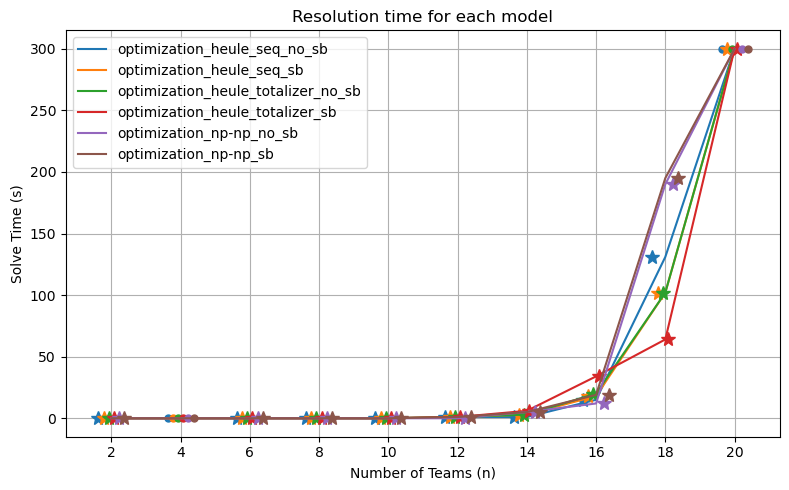
\includegraphics[width=\linewidth]{imgs/output.png}
        \caption{Resolution time}
    \end{subfigure}
    \caption{Runtimes for the optimization version of the Sports Tournament Scheduling (STS) problem. Data points are marked to indicate the solution status: a star ($\star$) indicates that a solution (optimal or sub-optimal) was found, while a circle ($\bullet$) indicates that no solution was found within the time limit.}
\end{figure}








     



\section{SMT Model}

\subsection{Decision Variables}

Let $n$ be the number of teams, and let $W = \{1, \dots, n - 1\}$ denote the set of tournament weeks. Each week is divided into $n/2$ periods. Let $\mathcal{M}_w$ be the set of matches scheduled in week $w \in W$.

We define an integer decision variable:
\[
p_{w,i,j} \in \{1, \dots, n/2\}
\]
for each match between any pair of teams $(i,j)$, where $(i,j) \in \mathcal{M}_w$, indicating the period during which this match takes place in week $w$.

The model is encoded using the theory of Linear Integer Arithmetic (LIA), extended with pseudo-Boolean constraints for cardinality.

\subsubsection{Pre-solving with the Circle Method}
\label{CircleMatching}

We avoid additional decision variables by precomputing which teams $(i, j)$ play in each week $w$ using the fast and classical \emph{circle method} for round-robin tournaments \cite{dewerra1999}, which was already explained above.
In practice, this greatly reduces the number of SMT variables and constraints. Thanks to pre-solving, we can solve instances with up to $n=20$ teams—and usually even $n=22$ sometimes — within the 5-minute limit. This is $2$ to $4$ teams more than our first SMT models that generated all possible matches as decision variables.

%One team (the pivot) is fixed, and the other $n - 1$ teams are placed in a circle. Each week, the pivot plays a rotating team, while the remaining teams are paired by connecting opposite positions in the circle. This rotation continues for $n - 1$ weeks. The construction guarantees:
%\begin{itemize}
%    \item Each team plays once per week;
%    \item No match is repeated;
%    \item The total number of matches is $\frac{n(n-1)}{2}$.
%\end{itemize}

%Example for $n = 6$:
%\[
%\text{Week 1: } (6,1), (2,5), (3,4) \quad \text{Week 2: } (6,2), (3,1), (4,5), \dots
%\]

% Mathematically, this yields a 1-factorization of the complete graph $K_n$, ensuring correctness. 

\subsection{Objective Function}

For the sake of solving the home-away balancing task, there is a simple mathematical algorithm. It does not need optimization with SMT.
If (i,j) is a game between any two teams $i$ and $j$ then the modulo arithmetic's algorithm is this:
\[
i,j\in\{1,\dots,n\},\quad
d\equiv j-i\pmod n,\;1\le d\le n-1,
\qquad
\text{home}(i,j)=
\begin{cases}
i,&d<\tfrac n2,\\
j,&d\ge\tfrac n2,
\end{cases}
% \quad
% \text{away}(i,j)=\text{the other vertex.}
\]
By construction, it achieves an absolute disbalance of home/away games equal to 1 per each team. In total, the sum of the absolute disbalance values will be n.
Theoretically, it is minimal for even n.

We use this mathematical approach in the decisional version, so the json results for the decisional version are also home/away optimal.

But to study the solver overhead of enforcing this balance via optimization, we performed a dedicated experiment. 
We define for team t - absolute difference between home and away games as:
\[
\mathit{abs\_diff}_t \;=\;\bigl\lvert (n-1)\;-\;2\cdot\mathit{away\_count}_t\bigr\rvert
\]
% equals 1 for every team, so that
% \[
% \sum_{t=1}^{n}\mathit{abs\_diff}_t \;=\;n,
% \]

 We introduced the global imbalance metric
\[
\texttt{sumDif} \;=\;\sum_{t=1}^{n}\mathit{abs\_diff}_t
\]
as our first attempt to construct an objective function.  Also, we added the constraint
\[
\texttt{sumDif} \;\ge\; n
\]

We added following additional symmetry‑breaking constraint (w.r.t to team numbering) on the per‑team imbalances:
\[
\mathit{abs\_diff}_{t_1}\;\ge\;\mathit{abs\_diff}_{t_2}\;\ge\;\cdots\ge\;\mathit{abs\_diff}_{t_n},
\]
and then instructed Z3 to minimize
\[
\max_{t}\mathit{abs\_diff}_t = abs\_diff_{0}
\]

In our experiments, it appeared that instead of minimizing $\texttt{sumDif}$, it is better to minimize $\max_{t}\mathit{abs\_diff}_t$ objective, as the optimization becomes almost an order of magnitude faster. 
\subsection{Constraints}

\paragraph{Domain Constraints.}
Each decision variable must be assigned a valid period:
\[
\forall (w,i,j): \quad 1 \leq p_{w,i,j} \leq n/2
\]

\paragraph{Unique Match per Period per Week.}
For each week $w \in W$ and period $k \in \{1, \dots, n/2\}$, exactly one match must be assigned to that period:
\[
\sum_{(i,j) \in \mathcal{M}_w} [p_{w,i,j} = k] = 1
\]

\paragraph{Period Load per Team.}
Each team must appear at most twice in each period across the tournament:
\[
\forall t \in [n], \forall k \in \{1, \dots, n/2\}: \quad \sum_{(w,i,j) : t \in \{i,j\}} [p_{w,i,j} = k] \leq 2
\]

\subsubsection*{Symmetry Breaking Constraints}

\paragraph{Fixed Periods in First Week.}
To reduce the search space, we fix the period assignment of all matches in the first week:
\[
\forall k \in \{1, \dots, n/2\},\quad p_{1,i_k,j_k} = k
\]
where $(i_k, j_k)$ is the $k$-th match in a lexicographically sorted list of matches in week 1. This removes the permutation symmetry for the period labels.

In our SMT tests more complicated constraints - like lexicographical constraints on period assignment vectors for chosen pairs of teams - did not bring any noticeable additional improvements, as well as adding redundant constraints. 

% \paragraph{Lexicographic Team Schedule Ordering.}
% Let $T_1$ and $T_2$ be the last two teams in lexicographic order. Let $\vec{v}_1$ and $\vec{v}_2$ be the sequences of period variables corresponding to matches involving $T_1$ and $T_2$, respectively. Then, we enforce:
% \[
% \vec{v}_1 \leq_{\text{lex}} \vec{v}_2
% \]
% This is encoded using a sequence of implications to ensure that if all earlier positions are equal, the first differing value in $\vec{v}_1$ must be less than or equal to the corresponding one in $\vec{v}_2$.

\subsection{Validation}

\paragraph{Solver.}
The model was implemented in Python using the Z3 SMT solver. A custom tactic pipeline was used to enable pseudo-Boolean cardinality constraints translation into bit-vector constraints for speed.
%\[
%\texttt{Then(`card2bv', `smt')}
%\]

\subsection*{Experimental Results (Decision version, SMT in Z3)}

We tested the SMT model (without home-away optimization) using Z3 on increasing values of $n$, with and without symmetry breaking. All runs were limited to 300 seconds. The results in Table~\ref{tab:smt-results} show that enabling symmetry breaking significantly improves performance, especially for larger instances.

\begin{table}[h!]
\centering
\caption{Runtime in seconds for SMT (decision version), Z3 solver, with and without symmetry breaking (SB).}
\label{tab:smt-results}
\begin{tabular}{|c|c|c|}
\hline
\textbf{Number of Teams} & \textbf{SB Enabled} & \textbf{SB Disabled} \\
\hline
6  & 0 & 0 \\
8  & 0 & 0 \\
10 & 0 & 0 \\
12 & 0 & 1 \\
14 & 0 & 0 \\
16 & 0 & 2 \\
18 & 8 & 17 \\
20 & 5 & 42 \\
\hline
\end{tabular}
\end{table}

For our SMT model, we observed that the simple version (first week periods were fixed) of symmetry breaking consistently reduced runtime for bigger $n$, especially beyond $n = 16$. Without SB, solving $n=20$ takes $8$ times longer.

Though we need to mention that for a fixed $n$ there is still some variation between runs - due to the solver's heuristic choices adding some randomness. In some cases $n = 22$ gets solved on our hardware, while often it times out, so it was not included in the final table.

\subsection*{Experimental Results (Optimization version, SMT in Z3)}

We extended the SMT model to solve the optimization version of the problem, where the objective is to minimize the maximal (w.r.t to all teams) absolute discrepancy in home/away balance. 
Theoretically, our objective - maximal absolute discrepancy - being equal to $1$ is equivalent to reaching the optimum, and indeed this optimum value was reached in all tested instances.
%For $n$ teams, the theoretical optimum for the sum of absolute discrepancies is $n$.  

Table~\ref{tab:smt-opt-results} reports the total solving time (in seconds) for various team sizes, both with and without symmetry breaking (SB). All runs were performed with Z3 under a 5-minute timeout. In all cases, the solver found and proved optimal solutions within the time limit.

\begin{table}[h!]
\centering
\caption{Runtime in seconds for SMT (optimization version), Z3 solver, with and without symmetry breaking (SB). The objective function, $\max_{t}\mathit{abs_diff}_t$, in every case was optimal, and the value is shown in bold.}
\label{tab:smt-opt-results}
\begin{tabular}{|c|c|c|}
\hline
\textbf{Number of Teams} & \textbf{SB Enabled} & \textbf{SB Disabled} \\
\hline
6  & 0.00\textbar\textbf{1} & 0.00\textbar\textbf{1} \\
8  & 0.00\textbar\textbf{1} & 0.00\textbar\textbf{1} \\
10 & 0.00\textbar\textbf{1} & 0.00\textbar\textbf{1} \\
12 & 3.00\textbar\textbf{1} & 6.00\textbar\textbf{1} \\
14 & 4.00\textbar\textbf{1} & 11.00\textbar\textbf{1} \\
16 & 127.00\textbar\textbf{1} & 44.00\textbar\textbf{1} \\
18 & 189.00\textbar\textbf{1} & 257.00\textbar\textbf{1} \\
20 & 149.00\textbar\textbf{1} & 154.00\textbar\textbf{1} \\
\hline
\end{tabular}
\end{table}

We observe that for the SMT optimization version, symmetry breaking has no such dramatic impact for bigger $n$, 
though it helped in every case except for $n = 16$. For $n = 12$ and $n = 14$, SB yields a $2$ times and $3$ times improvement.

Though there is a noticeable variance due to solver heuristic choices, the observations made above are true for the majority of the re-runs, if made. 

% \subsection*{Experimental Results (Optimization version, SMT in Z3)}

% We tested the SMT model (without home-away optimization) using Z3 on increasing values of $n$, with and without symmetry breaking. All runs were limited to 300 seconds. The results in Table~\ref{tab:smt-results} show that enabling symmetry breaking significantly improves performance, especially for larger instances.

    

\begin{thebibliography}{9}

\bibitem{dewerra1999}
Dominique de Werra.
\newblock Scheduling Round-Robin Tournaments: An Overview.
\newblock \emph{Discrete Applied Mathematics}, 91(1–3):241--277, 1999.

\bibitem{bailleux2003}
Olivier Bailleux and Yacine Boufkhad.
\newblock Efficient CNF Encoding of Boolean Cardinality Constraints.
\newblock In: \emph{Principles and Practice of Constraint Programming (CP 2003)}, Lecture Notes in Computer Science, 2003.
\end{thebibliography}

\end{document}
